	\documentclass[10pt,oneside]{CBFT_book}
	% Algunos paquetes
	\usepackage{amssymb}
	\usepackage{amsmath}
	\usepackage{graphicx}
	\usepackage{libertine}
	\usepackage[bold-style=TeX]{unicode-math}
	\usepackage{lipsum}

	\usepackage{natbib}
	\setcitestyle{square}

	\usepackage{polyglossia}
	\setdefaultlanguage{spanish}


	\usepackage{CBFT.estilo} % Cargo la hoja de estilo

	% Tipografías
	% \setromanfont[Mapping=tex-text]{Linux Libertine O}
	% \setsansfont[Mapping=tex-text]{DejaVu Sans}
	% \setmonofont[Mapping=tex-text]{DejaVu Sans Mono}

	%===================================================================
	%	DOCUMENTO PROPIAMENTE DICHO
	%===================================================================

\begin{document}

% =================================================================================================
\chapter{Conceptos fundamentales de electromagnetismo}
% =================================================================================================


% =================================================================================================
\section{Ecuaciones de Maxwell}
% =================================================================================================

Son ecuaciones lineales de modo que vale la superposición (con \vb{E}, \vb{B} y 
cualquier vector relacionado linealmente con ellos).
\[
	\nabla \cdot \vb{D} = 4 \pi \rho_\ell \qquad \nabla \cdot \vb{B} = 0
\]
\[
	\nabla \times \vb{E} = - \frac{1}{c} \dpar{B}{t} \qquad \nabla \times \vb{H} =
	\frac{4\pi}{c} \vb{J}_\ell + \frac{1}{c}\dpar{D}{t}
\]
\[
	\vb{F} = q \left( \vb{E} + \frac{1}{c} \vb{v} \times \vb{B} \right)
\]

Los vectores pueden ser polares (tienen físicamente bien definido el sentido) o
axiales (se les atribuye un sentido por convención).

Las ecuaciones son invariantes ante transformaciones del tipo: rotación
y reflexión espacial y temporal.

% =================================================================================================
\section{Electrostática}
% =================================================================================================

La ley de Coulomb reza que
\[
	\vb{F}_{12} = q_1 q_2 \frac{(\vb{x}_1 - \vb{x}_2)}{|\vb{x}_1 - \vb{x}_2 |^3}
\]
que es la fuerza sobre 1 debido a 2. De la ley de Coulomb se puede definir 
\[
	\vb{E}_{12}(\vb{x}_1) \equiv \vb{F}_{12}/q_1
\]
y tomando $\vb{x}_1 \equiv \vb{x}$ y haciendo el límite $q_1 \to 0$ se tiene
\[
	\vb{E}(\vb{x}) = \sum_{i=1}^N \; q_i \frac{(\vb{x} - \vb{x}_i)}{|\vb{x} - \vb{x}_i |^3}
\]
que es el campo eléctrico y que en el paso al continuo resulta
\[
	\vb{E}(\vb{x}) = \int_{V'} \rho(\vb{x}) \frac{(\vb{x} - \vb{x}_i)}{|\vb{x} - \vb{x}_i |^3} dV' 
\]
siendo \vb{x} punto campo y $\vb{x}_i$ punto fuente.

\begin{figure}[htb]
	\begin{center}
	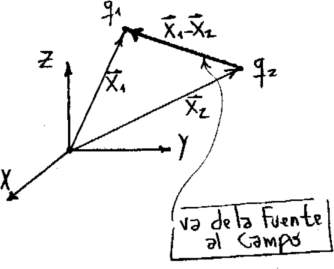
\includegraphics[width=0.6\textwidth]{images/fig_ft1_ejescargas.pdf}	 
	\end{center}
	\caption{}
\end{figure} 

\subsection{Conservación de la carga}

La carga total sale de una integral 
\[
	Q = \int_{V'}  \rho(\vb{x}') dV'
\]
como muestra la imagen
\begin{figure}[htb]
	\begin{center}
	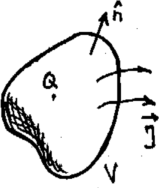
\includegraphics[width=0.25\textwidth]{images/fig_ft1_conserv.pdf}	 
	\end{center}
	\caption{}
\end{figure} 
y si el volumen es fijo podemos tomar la derivada con respecto al tiempo que pasa el interior como
derivada parcial,
\[
	\dtot{Q}{t} = \int_{V'} \dpar{\rho}{t} (\vb{x}') dV' = - \int_{S\equiv\partial V'} \vb{J} \cdot d\vb{S}
\]
y el miembro extremo derecho  se debe a que si la carga varía es a consecuencia de que se va en
forma de flujo. Aplicando el teorema de la divergencia en el miembro derecho,
\[
	\int_{V'} \dpar{\rho}{t} (\vb{x}') dV' = - \int_{V'} \nabla \cdot \vb{J} \; dV'
\]
lo cual vale para todo volumen y entonces esto significa que
\[
	\dpar{\rho}{t} + \nabla \cdot \vb{J} = 0
\]
que es la ecuación de continuidad de la carga. Si fuera $\nabla \cdot \vb{J}=0$ esto significa que las líneas
de \vb{J} no tienen principio ni fin.

% =================================================================================================
\section{Interacción magnética}
% =================================================================================================

Cuando se da $\nabla \cdot \vb{J}=0$ hablamos de una corriente estacionaria (no hay acumulación de carga en
ninguna parte). Las corrientes estacionarias producen efectos magnéticos dados por la ley de Biot-Savart
\[
	\vb{B}(\vb{x}) = \frac{1}{c} \int_\Gamma \frac{I d\vb{\ell}' \times (\vb{x} - \vb{x}')}{|\vb{x} - \vb{x}'|^3} 
\]
que es válida para un circuito $\Gamma$, que es una curva que se recorre en sentido CCW.
En el caso de un volumen la expresión es


% =================================================================================================
\section{Teorema de Helmholtz}
% =================================================================================================


% =================================================================================================
\section{Ley de Gauss}
% =================================================================================================

\begin{figure}[htb]
	\begin{center}
	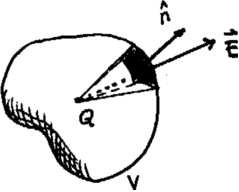
\includegraphics[width=0.6\textwidth]{images/fig_ft1_gauss.pdf}	 
	\end{center}
	\caption{}
\end{figure} 


\begin{figure}[htb]
	\begin{center}
	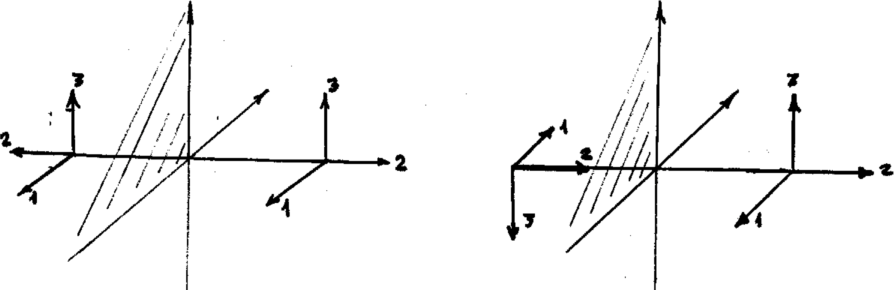
\includegraphics[width=0.6\textwidth]{images/fig_ft1_reflexvect.pdf}	 
	\end{center}
	\caption{}
\end{figure} 

% \bibliographystyle{CBFT-apa-good}	% (uses file "apa-good.bst")
% \bibliography{CBFT.Referencias} % La base de datos bibliográfica

\end{document}
